\section{Аналитическая часть}
\subsection{Нечеткая логика}
\subsubsection{Нечеткие множества}
Характеристическая функция, описывающая принадлежность элемента четкому множеству, выглядит следующим образом:
\begin{equation}
\mu_{A}^*(x) = \left \{ \begin{array}{ll}
1, x \in A\\
0, x \notin A
\end{array} \right.
\end{equation}

Графическая форма принадлежности $x$ четкому множеству $A$ представлено на рисунке \ref{fig:binary}.
\begin{figure}[H]
	\centering
	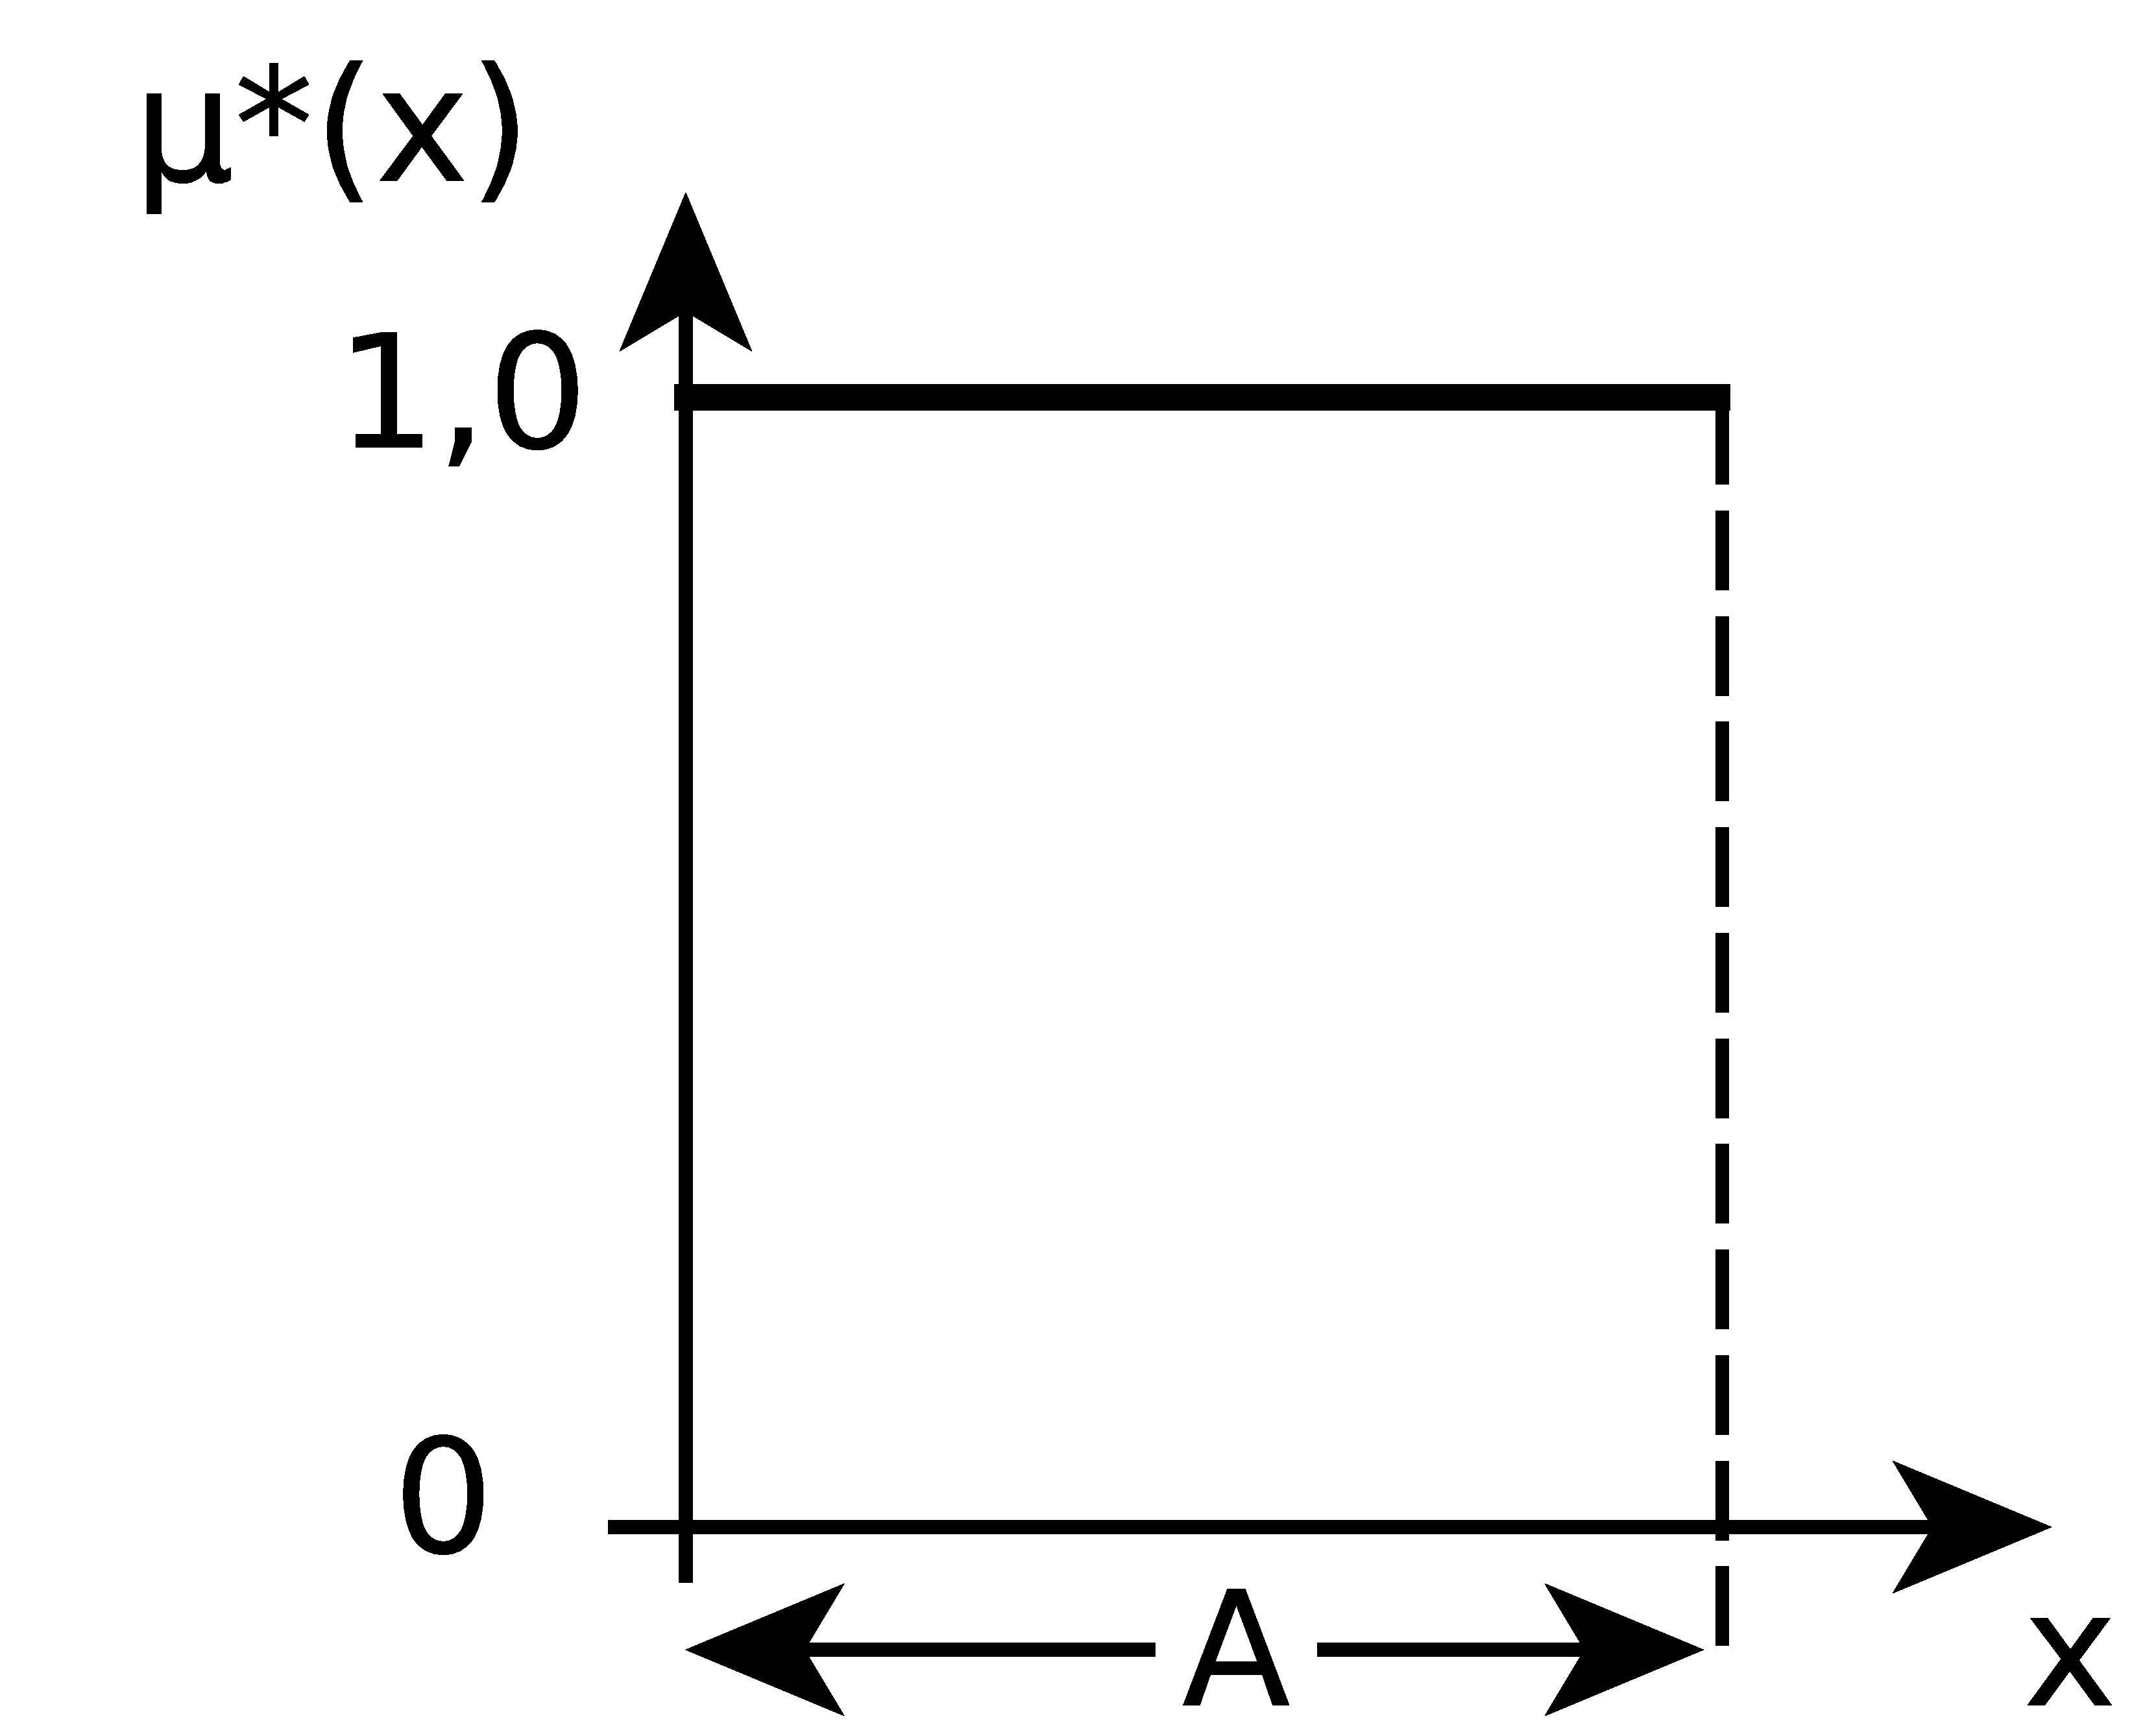
\includegraphics[width=0.4\linewidth]{img/binary}
	\caption{Принадлежность элемента четкому множеству}
	\label{fig:binary}
\end{figure}

В теории нечетких множеств $\mu_{A}(x)$ -- одномерная функция принадлежности, если область значений одномерного отображения $\mu_{A}(x) \in [0,1]$, пример ее графической формы представлен на рисунке \ref{fig:fuzzy}.
\begin{figure}[H]
	\centering
	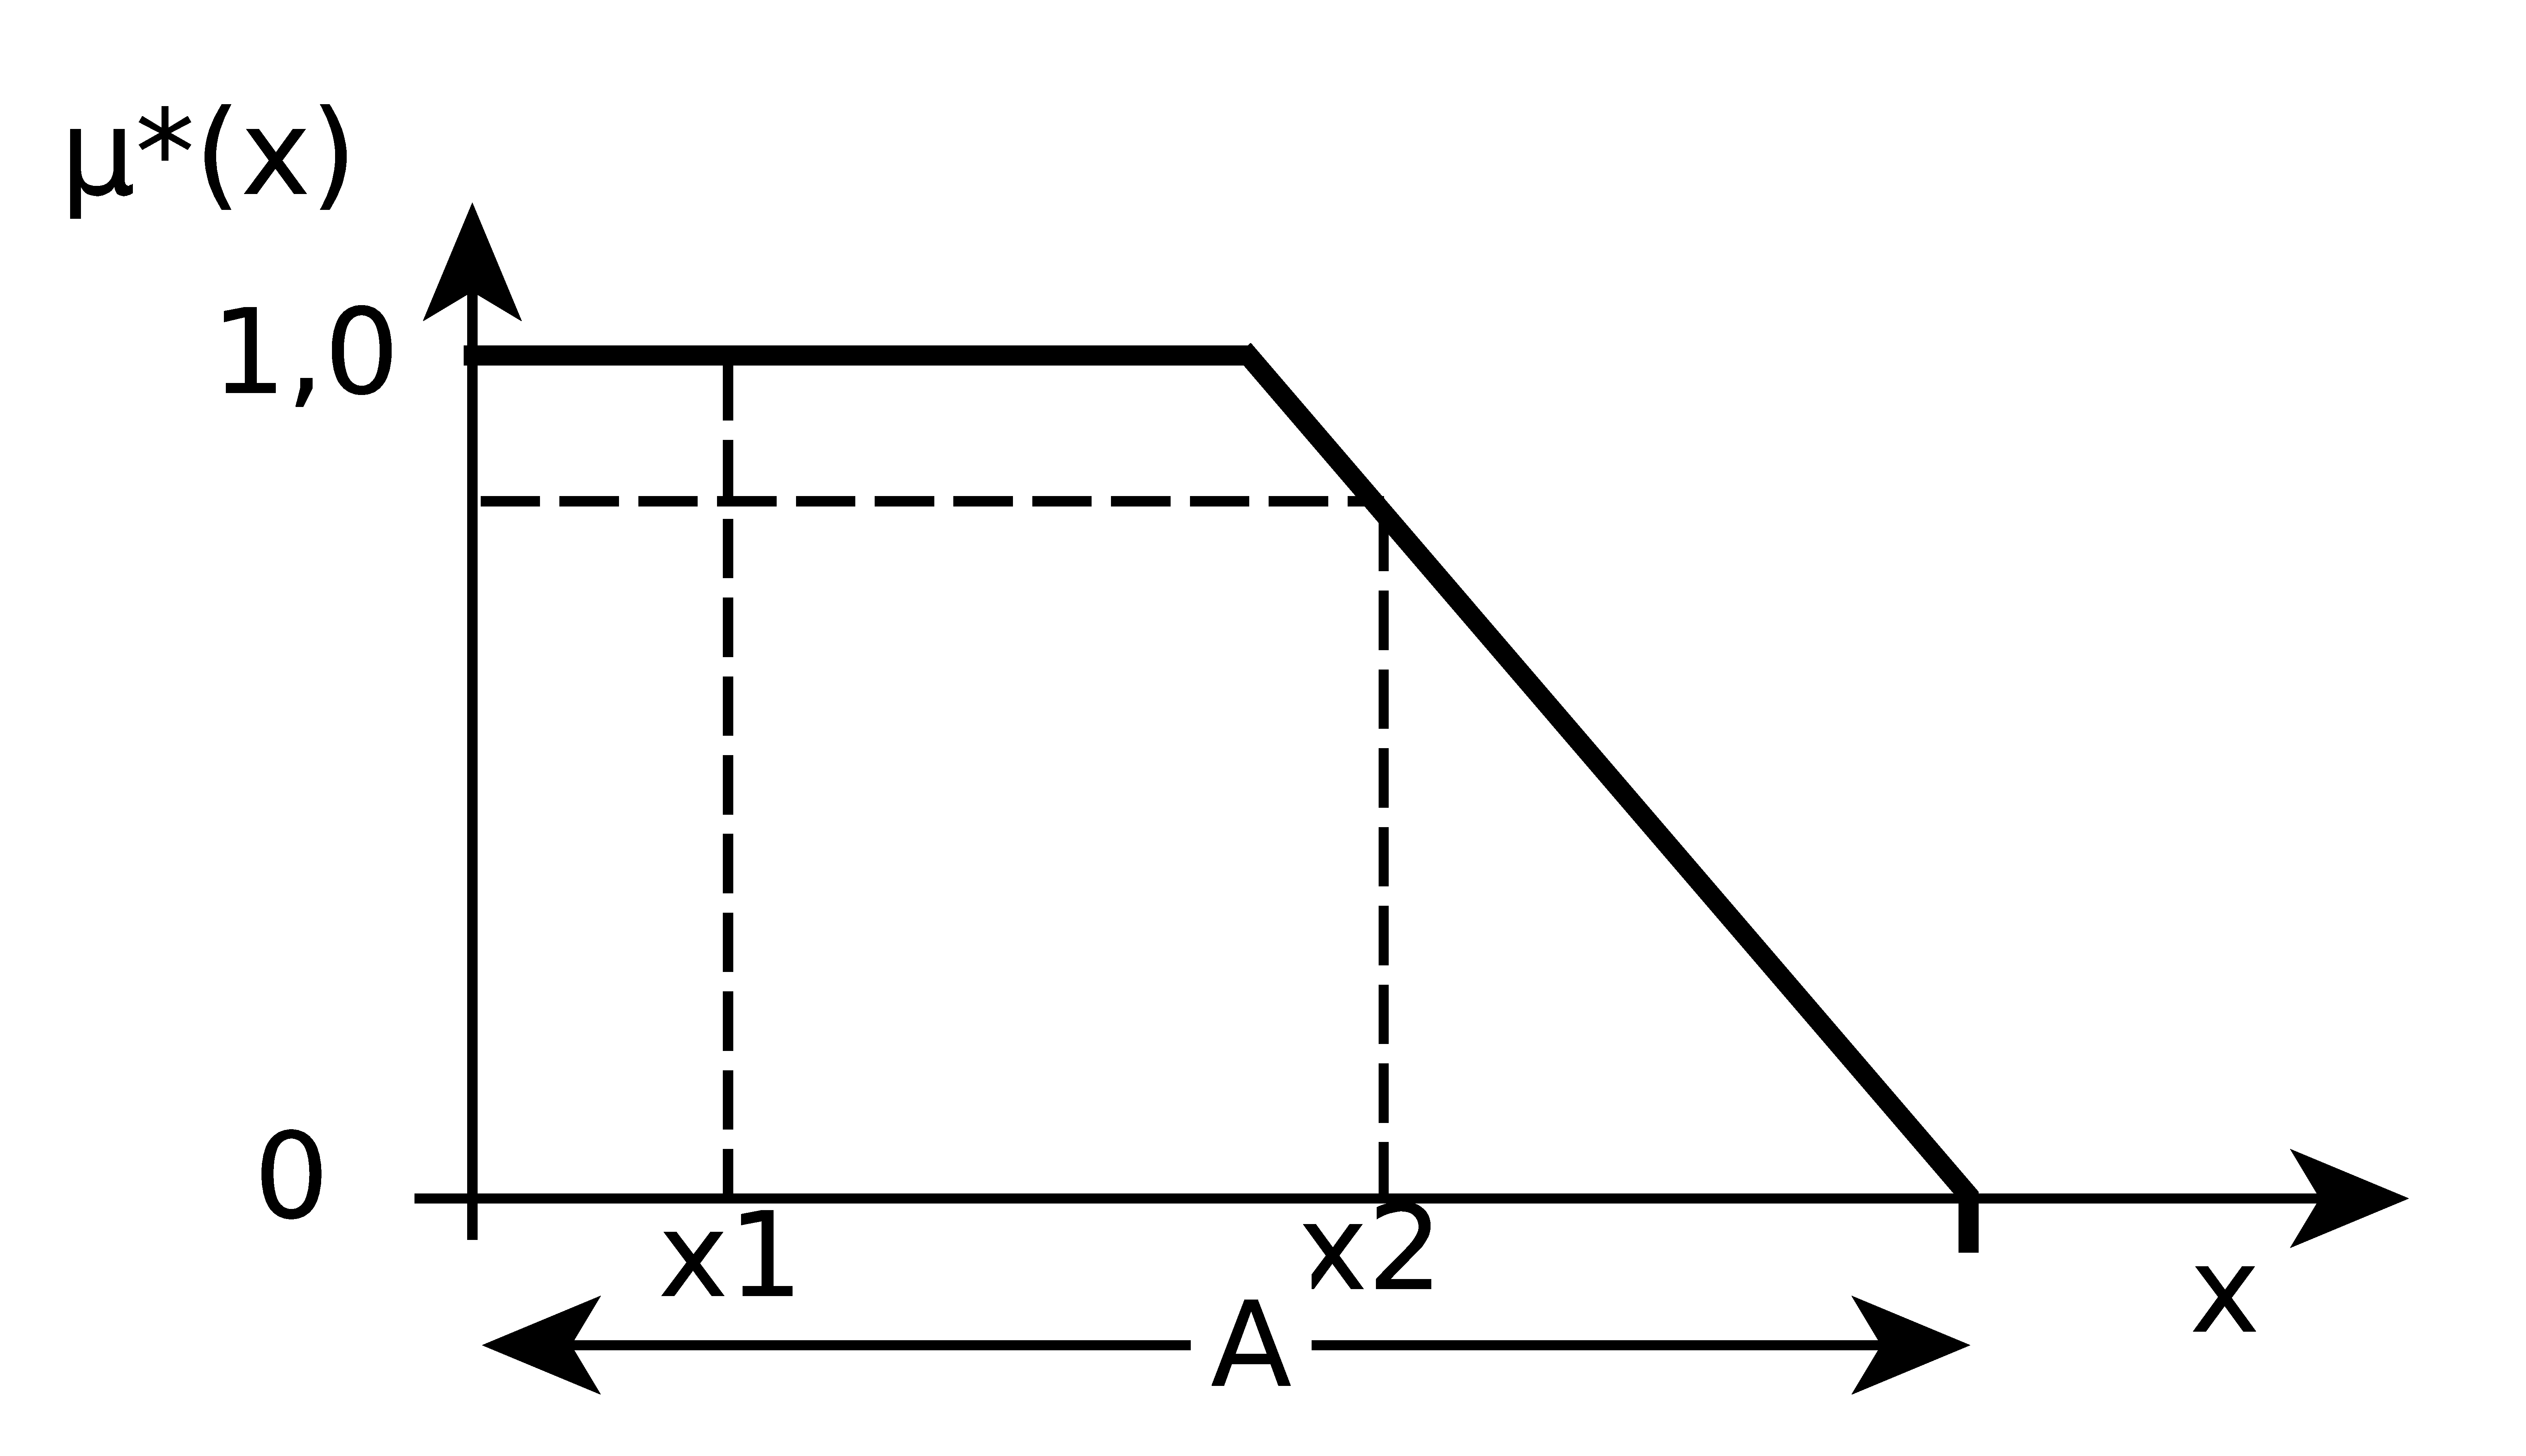
\includegraphics[width=0.6\linewidth]{img/fuzzy}
	\caption{Принадлежность элемента нечеткому множеству}
	\label{fig:fuzzy}
\end{figure}

Наиболее часто используемыми функциями принадлежности являются следующие:
\begin{itemize}
	\item трапециевидная: 
	\begin{equation}
	\label{eq:tr-func}
		\mu(x; a, b, c, d) = \left\{
		\begin{aligned}
			&0, x \leqslant a,\\
			&\cfrac{x-a}{b-a}, \hfill a < x \leqslant b,\\
			&1, \hfill b < x \leqslant c,\\
			&\cfrac{d-x}{d-c}, \hfill c < x \leqslant d,\\
			&0, \hfill d < x;
		\end{aligned} \right.
	\end{equation}
	\item треугольная:	
	\begin{equation}
	\label{eq:triangle-func}
		\mu(x;a, b, c) = \left\{
		\begin{aligned}
			&0, x \leqslant a,\\
			&\cfrac{x-a}{b-a}, a < x \leqslant b,\\
			&\cfrac{c-x}{c-b}, b < x \leqslant c,\\
			&0, c < x;
		\end{aligned}
		\right.
	\end{equation}
	\item S-функция:	
	\begin{equation}
	\label{eq:S-func}
		S(x;\alpha, \beta, \gamma) = \left\{
		\begin{aligned}
			& 0, x \leqslant \alpha,\\
			& 2\cdot \left(\cfrac{x-\alpha}{\gamma-\alpha}\right)^2, \alpha < x \leqslant \beta,\\
			&1 - 2\cdot \left(\cfrac{\gamma-x}{\gamma-\alpha}\right)^2, \beta < x \leqslant \gamma,\\
			&1, \gamma < x;
		\end{aligned}
		\right.
	\end{equation}
	\item $\Pi$-функция:	
	\begin{equation}
	\label{eq:P-func}
		\Pi(x;\beta, \gamma) = \left\{
		\begin{aligned}
			& S(x; \gamma - \beta, \gamma - \frac{\beta}{2}, \gamma), x \leqslant \gamma,\\
			& 1 - S(x; \gamma, \gamma + \frac{\beta}{2}, \gamma + \beta), \gamma < x;
		\end{aligned}
		\right.
	\end{equation}
	\item лингвистическая функция (результат применения лингвистического барьера (<<Очень>>, <<Не>>, <<Более или менее>>, прочее) к функции принадлежности множества), например:
	\begin{itemize}  
		\item Очень A:
		 \begin{equation}
			\mu_{Very A}(x) = CON(A) = \mu_A(x)^2;
			\end{equation}
		\item Более или менее A:
		 \begin{equation}
		\mu_{More or Less A}(x) = DIL(A) = \mu_A(x)^{0.5};
		\end{equation}
		\item Не A:
		 \begin{equation}
		\mu_{Not A}(x) = 1 - \mu_A(x);
		\end{equation}
		\item Не Очень A:
		 \begin{equation}
		 \label{eq:notVery}
		\mu_{Not Very A}(x) = 1 - CON(A).
		\end{equation}
	\end{itemize}
\end{itemize}

Нечеткой переменной называется тройка
\begin{equation}
\{X, U, \widetilde{A}\},
\end{equation}
где $X$ -- вербальное название переменной, $U$ -- область ее определения (универсальное множество), $\widetilde{A}$ -- нечеткое множество универсального множества, описывающее возможные значения нечеткой переменной \cite{IncrEfficiency}.

Основные операции над нечеткими множествами \cite{FuzRegul}--\cite{ExpSystems}:
\begin{itemize}
	\item объединение:
	\begin{equation}
	\label{eq:cup}
	A \cup B: \mu_{A \cup B}(x) = \max(\mu_A(x), \mu_B(x));
	\end{equation}
	\item пересечение:
	\begin{equation}
	\label{eq:cap}
	A \cap B: \mu_{A \cap B}(x) = \min(\mu_A(x), \mu_B(x));
	\end{equation}
	\item отрицание:
	\begin{equation}
	\label{eq:neg}
	\bar A: \mu_{\bar A}(x) = 1 - \mu_{A}(x);
	\end{equation}
	\item концентрация:
	\begin{equation}
	\label{eq:con}
	CON(A): \mu_{CON(A)}(x) = (\mu_A(x))^2;
	\end{equation}
	\item растворение:
	\begin{equation}
	\label{eq:dil}
	DIL(A): \mu_{DIL(A)}(x) = (\mu_A(x))^{0.5}.
	\end{equation}
\end{itemize}

\subsubsection{Лингвистические переменные}
Для количественной оценки смысла предложений естественного языка применяются нечеткие множества и лингвистические переменные, после чего появляется возможность манипулировать этими предложениями. Лингвистическим переменным присваиваются значения, представляющие собой такие выражения, как слова, фразы или предложения естественного или искусственного языка.

Лингвистическая переменная определяется следующим образом:
\begin{equation}
\{X, T(X), U, V, S\},
\end{equation}
где $X$ -- вербальное название переменной, $T(X) = \{X_{i}, i=\overline{1, m}\}$ -- терм-множество переменной X, т.~е. множество термов, или названий лингвистических значений (каждое из этих значений -- нечеткая переменная со значениями из универсального множества $U$), $V$ -- синтаксическое правило, которое ставит в соответствие каждой нечеткой переменной с названием из $T(X)$ нечеткое подмножество универсального множества $U$, $S$ -- семантическое правило, которое ставит в соответствие каждой нечеткой переменной с названием из $T(X)$ нечеткое подмножество универсального множества $U$ \cite{IncrEfficiency}.

\subsubsection{Экспертные системы}
Общая схема работы нечетких экспертных систем представлена на рисунках \ref{fig:expsys0}, \ref{fig:expsys1}.
\begin{figure}[H]
	\centering
	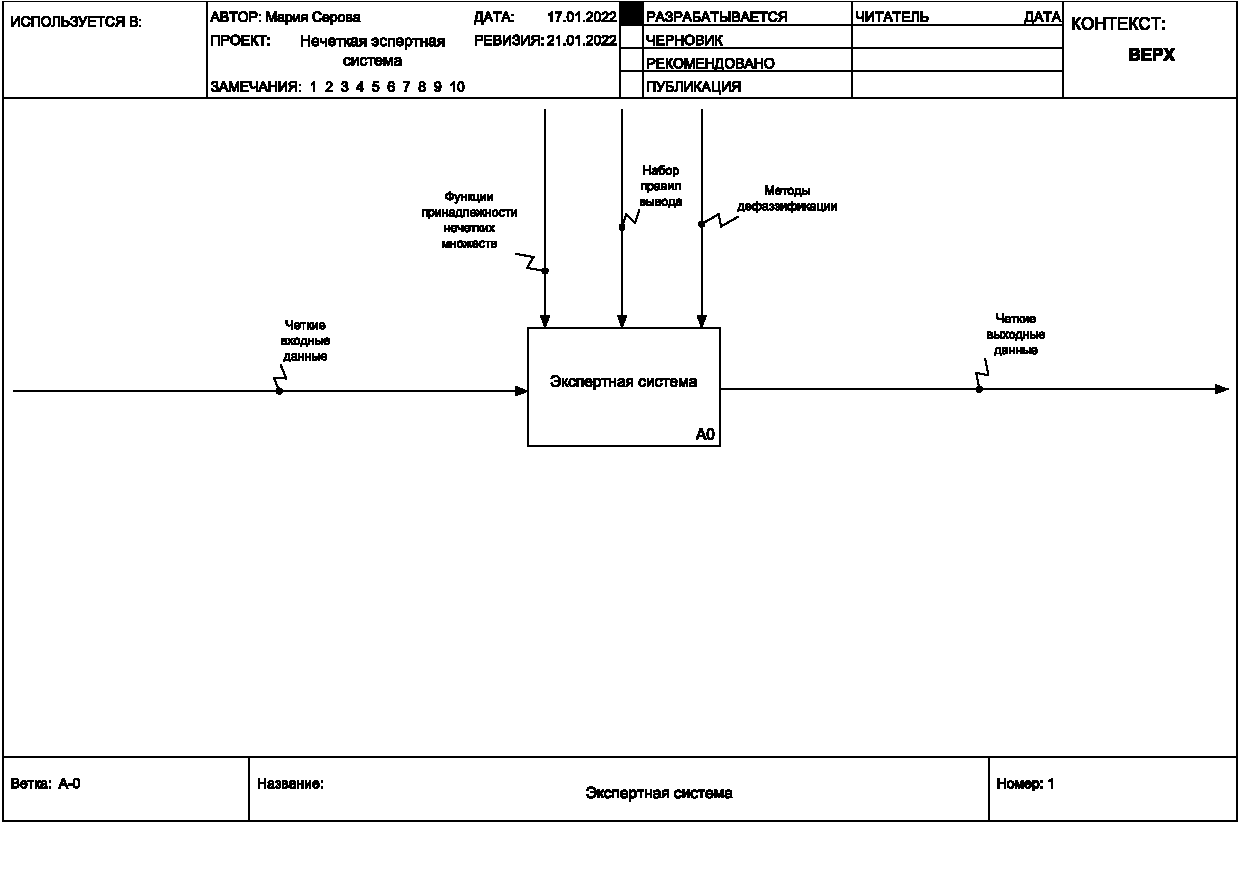
\includegraphics[width=0.75\linewidth]{img/expsys0}
	\caption{Схема работы экспертной системы}
	\label{fig:expsys0}
\end{figure}

\begin{figure}[H]
	\centering
	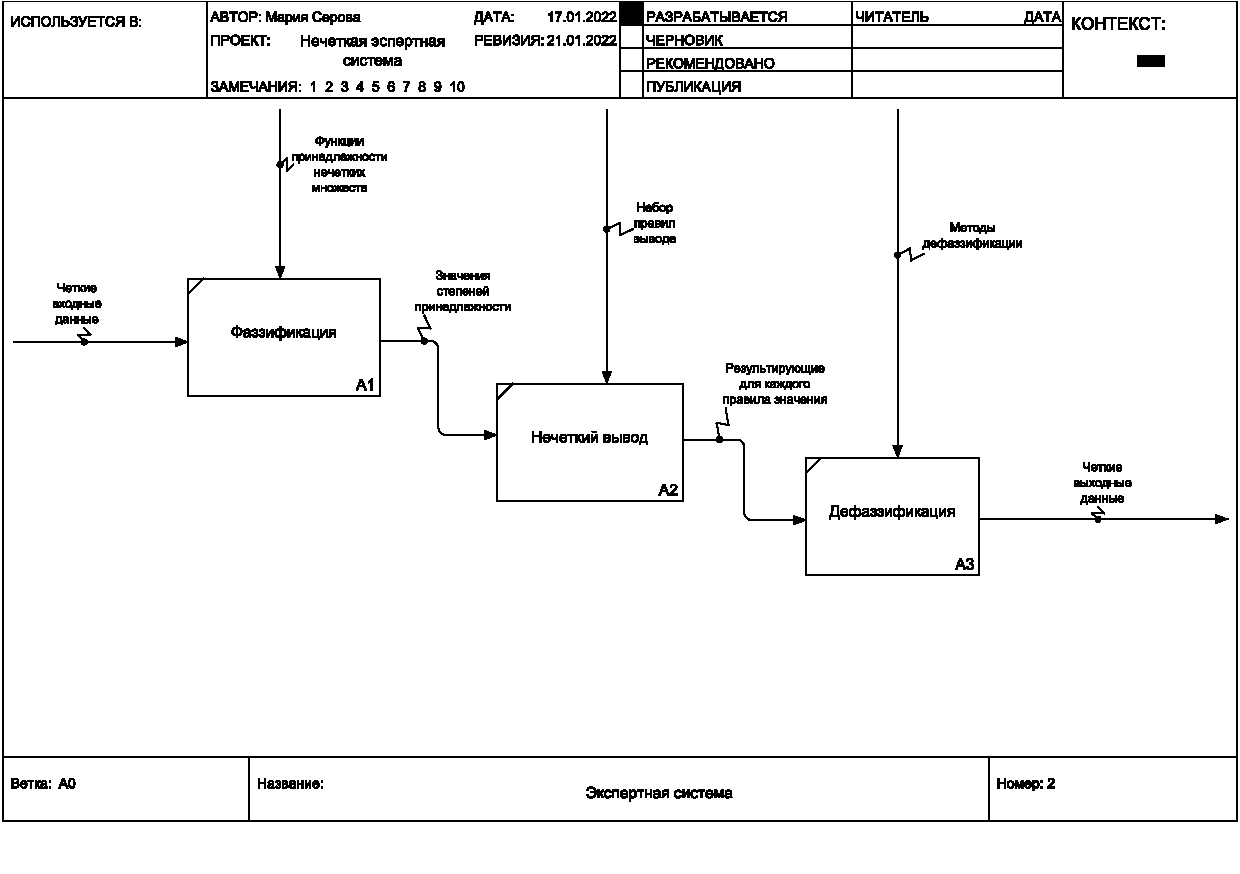
\includegraphics[width=0.75\linewidth]{img/expsys1}
	\caption{Этапы работы экспертной системы}
	\label{fig:expsys1}
\end{figure}

Работа любой нечеткой экспертной системы состоит из трех основных этапов \cite{SettingMamdani}:
\begin{itemize}
	\item фаззификация: четкие значения входных переменных $x$ приводятся к 
	
	нечетким значениям посредством вычисления их степени истинности выражения: $x_u$ есть $A_u^j$ как вычисления значения соответствующего значения входной функции принадлежности $\mu_A(x_u)$, где $u$ – номер входной переменной, $j$ – номер правила нечеткого логического вывода.
	\item нечеткий вывод: используя полученные на первом этапе значения степеней истинности, вычисляются результирующие значения для каждого $j$-го правила, вид которых определяется используемым механизмом нечеткого вывода, из набора в $m$ правил.
	\item дефаззификация: получение четкого значения.
\end{itemize}

Наиболее распространенные механизмы нечеткого логического вывода, которые легли в основу соответствующих типов экспертных систем \cite{SettingMamdani}--\cite{MultifuncImit}:
\begin{itemize}
	\item метод Мамдани: 
	\begin{equation}
	\label{eq:Mamdani}
	if(x_1~is~A_1^j)~...~and~(x_n~is~A_n^j)~then~y~is~B_k^j,
	\end{equation}
	где $and$ – операция пересечения нечетких множеств, k – номер функции принадлежности.
	\item метод Такаги--Сугено: 
	\begin{equation}
	if(x_1~is~A_1^j)~...~and~(x_n~is~A_n^j)~then~y=f(x_1,x_2, ..., x_n)=p_0+\sum_{i=1}^{n}p_ix_i.
	\end{equation}
\end{itemize}

Существует несколько методов для определения истинности консеквентов правила (дефаззификации) \cite{FuzRegul}--\cite{ExpSystems}:
\begin{itemize}
	\item метод максимума, при котором осуществляется выбор элемента с максимальной степенью принадлежности;
	\item метод моментов, при котором значения истинности консеквентам правил присваиваются с применением способа, аналогичному аналогичного способу вычисления первого момента инерции материального объекта в физике.
	\item метод центра тяжести;
	\item метод среднего максимума;
	\item метод центра области.
\end{itemize}

\subsection{Существующие решения}
При работе с нечеткими экспертными системами необходимо хранить переменные, функции принадлежности и продукционные правила. Можно выделить 2 подхода к хранению лингвистических переменных, функций принадлежности и продукционных правил:
\begin{itemize}
	\item в оперативной памяти;
	\item в базе данных.
\end{itemize}

Первый подход применим только для небольших стабильных систем, поскольку увеличение/изменение продукционных правил может привести к значительному изменению кода и ухудшению его восприятия, а увеличение количества лингвистических переменных и функций принадлежности будет ограничено размером оперативной памяти.
В связи с этим для работы с крупными экспертными системами прелоагается использовать базу данных.

В существующих решениях предлагается хранить в базах данных только лингвистические переменные и их функции принадлежности. Одни авторы \cite{Sorokin} предлагают хранить функции в виде точек (получаемая таким образом ломаная линия позволяет задавать функции любого вида), что не позволяет учитывать такие функции, как лингвистические, и требует ручного ввода точек. Другие авторы \cite{Mongo} отмечают возможность хранения информации о нечетких множествах в виде xml/json полей в таблице, однако в таком случае существует риск нарушения целостности базы данных из-за невозможности автоматической проверки, также подобный подход усложняет процесс работы с информацией. 

В работе \cite{StoringFuzzyNums} предлагается хранить нечеткие числа в виде кортежей \\*вида \ref{eq:cort}.
\begin{equation}
\label{eq:cort}
\begin{array}{l}
<PK, FK_1, FK_2, ..., FK_n, Data_1, Data_2, ..., Data_m, T, Max, \\
x1, x2, x3, x4>,
\end{array} 
\end{equation}

где $PK, FK_1, FK_2, ..., FK_n$ -- первичные и внешние ключи базы данных, $Data_1$, $Data_2$, ..., $Data_m$ -- атрибуты отношения (четкие данные), $T$ -- тип функции принадлежности, $Max$ -- максимальное значение функции принадлежности, $x_1, x_2, x_3, x_4$ -- аргументы функции принадлежности.

Данный подход не позволяет учитывать лингвистические и зависящие от других переменных функции. Также объединение нечетких переменных с функциями принадлежности, задающими нечеткое множество, приводит к дублированию информации.

\begin{figure}[H]
	\centering
	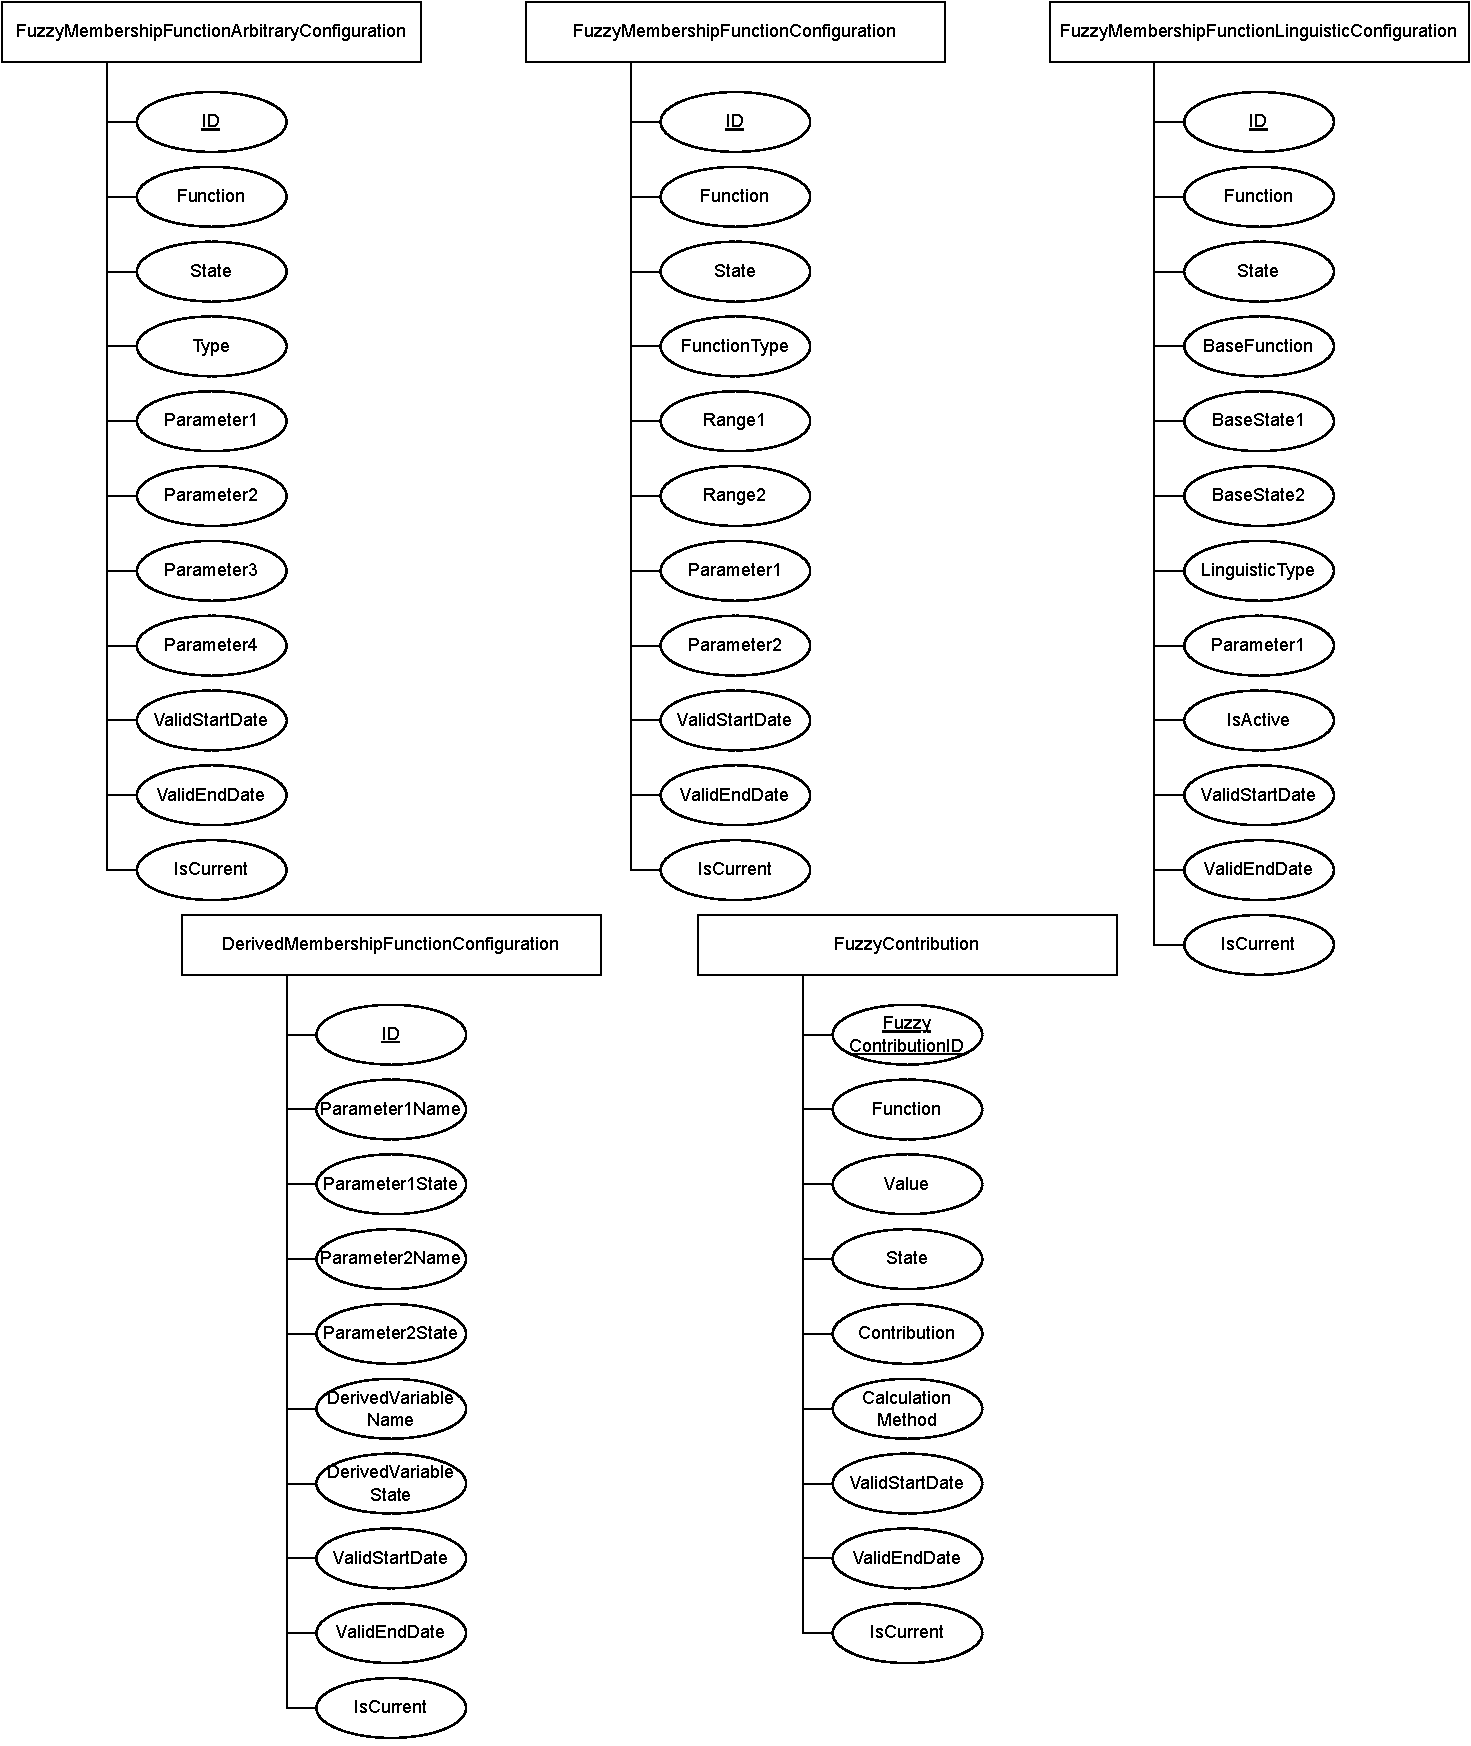
\includegraphics[width=0.95\linewidth]{img/Existing1}
	\caption{Сущности, предложенные Динешем Асанка и Амалем Перера}
	\label{fig:existing1}
\end{figure}

Предложенные в работе \cite{DefiningFuzz} сущности базы данных представлены на рисунке \ref{fig:existing1}. Авторы предлагают использовать отдельные таблицы для хранения информации о разных видах функций принадлежности, таких как обычная, \\*формируемая на основе данных, дифференциальная и лингвистическая. При этом данная система за счет полей ValidStartDate и ValidEndDate позволяет хранить историю изменений. Обычная функция принадлежности может иметь до четырех параметров, поскольку среди наиболее распространенных ее видов \\*(треугольная, $\Pi$-функция, проч.) максимальное количество аргументов (четыре) принимает трапециевидная. Для увеличения эффективности за счет однократного вычисления значения функции принадлежности для конкретной переменной предложена сущность FuzzyContribution, которая связывает лингвистическую переменную и функцию принадлежности.

Предложенная схема имеет следующий недостаток: хранение информации о функциях принадлежности в разных таблицах не позволяет ссылаться в одном поле переменной на необходимую функцию. Следовательно, возникает необходимость объединения различных параметров функций в одну таблицу. 

%Это можно обеспечить путем добавления допустимых типов функций принадлежности, сокращения количества используемых параметров (например, убрать поля State, IsCurrent и проч.), объединения нескольких параметров в 1.
% В нечетких экспертных системах функция принадлежности, зависящая от нескольких переменных, возникает только в результате срабатывания нечеткого правила, поэтому будем рассматривать их как несколько функций, зависящих от одной переменной, и свяжем их с одним консеквентом.

Авторы работы \cite{FuzzDb} предлагают создавать отдельные таблицы для каждой возможной функции принадлежности, в которых содержатся только необходимые для вычисления параметры. При этом переменная, относительно которой происходит вычисление функции принадлежности (например, лингвистической) хранится в таблице FuzzyValue (нечеткая переменная), как и тип используемой функции. Предлагаемая схема представлена на рисунке \ref{fig:existing2}.

Данная схема имеет несколько недостатков:
\begin{itemize}
	\item числовое значение нечеткой переменной является ее идентификатором, из-за этого отсутствует возможность разделять переменные каким-либо образом или создавать разные переменные с одинаковым значением;
	\item отсутствие лингвистических переменных не позволяет учитывать \\*возможность анализа принадлежности значения нескольким нечетким \\*множествам;
	\item сложность поиска данных: таблица, к которой должно производиться обращение, зависит от описанного в поле типа;
	\item значение функции принадлежности должно вычисляться каждый раз при обращении к данным.
\end{itemize}

\begin{figure}[H]
	\centering
	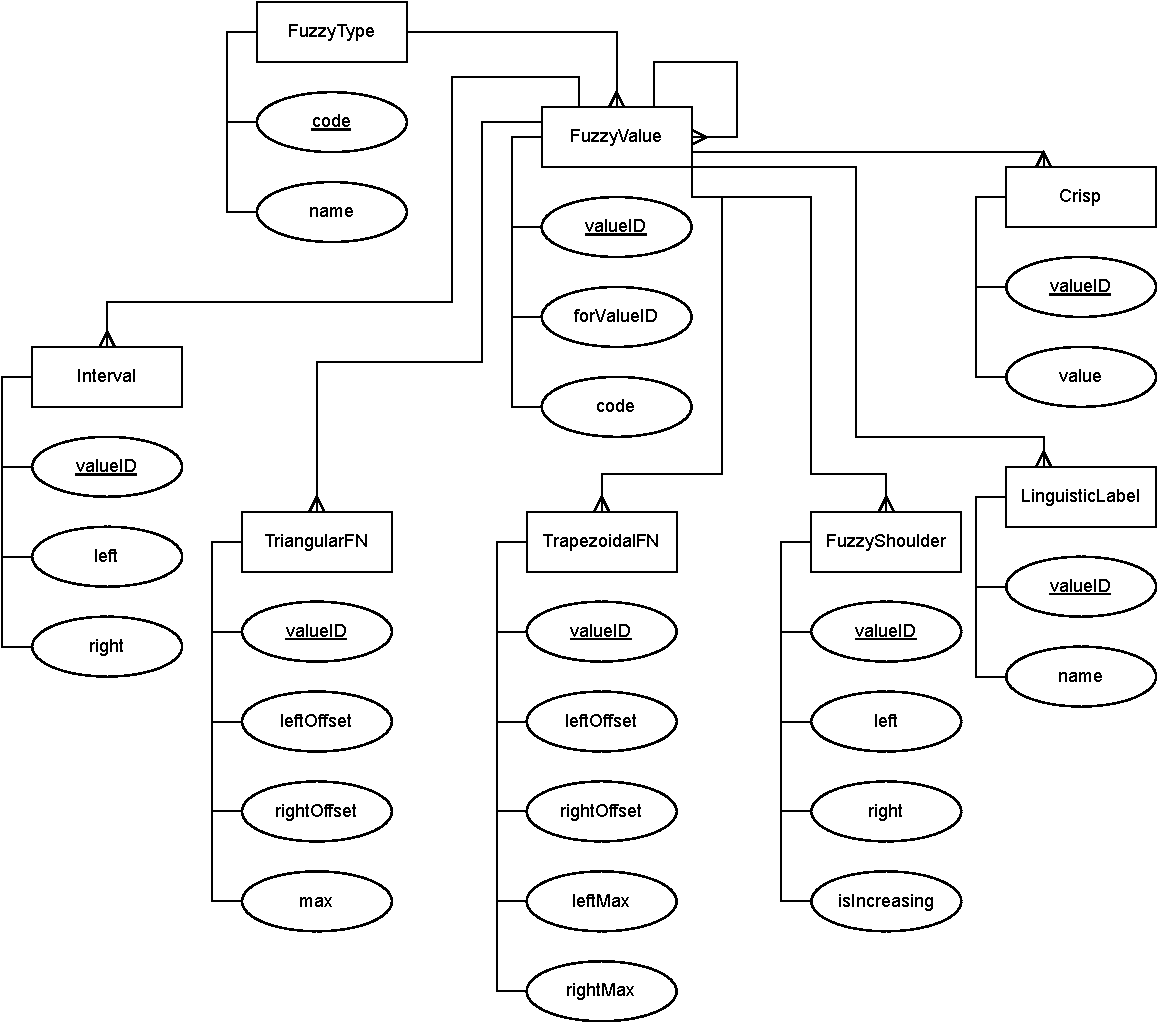
\includegraphics[width=0.85\linewidth]{img/Existing2}
	\caption{Модель базы данных, предложенная Срджаном Шкрибич и Милошем Ракович}
	\label{fig:existing2}
\end{figure}

\subsection{Базы данных и системы управления базами данных}
Для хранения больших объемов информации о нечетких экспертных системах используются базы данных. Для управления базами данных существуют системы управления базами данных (СУБД) -- совокупность программных, языковых и прочих средств, предназначенных для создания, управления, контролирования, администрирования и совместного использования базы данных разными пользователями \cite{OverviewComparativeDMS}.

\subsubsection{Классификация баз данных}
Все системы управления базами данных по модели хранения делятся на 3 типа, представленных ниже.
\begin{enumerate}
	\item Дореляционные \cite{DBIngeneering}:
		\begin{enumerate}
			\item Основанные на иерархической модели -- инвертированной древообразной структуры, в которой все узлы связываются друг с другом указателями.
			
			Преимущества подобного хранения данных заключаются в простоте понимания структуры, целостности, независимости и безопасности данных. Недостатками являются ограничения в отношениях между сущностями (невозможно создать отношения типа многие ко многим), структурная зависимость (данные также хранятся в виде дерева, при серьезных изменениях существует вероятность потери возможности навигации по данным) и сложность разработки прикладного ПО.
			
			\item Основанные на сетевой модели -- графовая структура.
			
			Данная модель позволяет назначать неограниченное количество связей между узлами графа и не требует переподчинения дочерних узлов при удалении узла, однако большое количество связей повышает сложности схемы и усложняет обеспечение целостности данных и разработку ПО.
		\end{enumerate}
	\item Реляционные. Данные хранятся в структурированном виде в таблицах, которые могут быть связаны с другими таблицами через внешние ключи \cite{OverviewDMS}. Такой подход требует тщательного анализа и выделения сущностей и связей между ними. Главными достоинствами реляционной модели являются целостность данных и соблюдение принципов ACID (атомарность, надежность, изолированность и долговечность) \cite{relativeNonRelative}, однако в процессе нормализации с целью устранения избыточности данных появляется много таблиц, соединение которых для получения информации требует больших временных затрат \cite{DBIngeneering}. Для работы с реляционными базами данных используется язык структурированных запросов SQL.
	\item Постреляционные (к таким СУБД относятся нереляционные) \cite{DBIngeneering}--\cite{relativeNonRelative}. Позволяют хранить неструктурированные данные, не имеют общего формата. К нереляционным относятся хранилища типа <<ключ-значение>> и базы данных, основанные на документ-ориентированной, графовой или столбцовой моделях. Основные преимущества данных СУБД заключаются в отсутствии необходимости предварительного структурирования данных, низких затратах на сборку в единое целое и простоте масштабирования, однако за это приходится платить ограниченностью синтаксических конструкций, разными языками для взаимодействия с каждой отдельной БД и возможностью потерей данных из-за ошибок.
\end{enumerate}
%
%\subsubsection{Реляционные СУБД}
%Наиболее распространенными реляционными СУБД на сегодняшний день являются Oracle, MySQL, PostgreSQL и SQLite.
%
%Oracle предназначена для применения в облачных средах и может быть размещена раздельно на нескольких серверах. Каждая транзакция выполняется изолированно от других, что обеспечивает безопасность данных. Для управления базами данных используются новейшие технологии. Данная СУБД является коммерческой, но имеет свободно распространяемые версии \cite{OverviewComparativeDMS}.
%% и на текущий день недоступна для приобретения на территории Российской Федерации.
%
%MySQL позволяет работать с данными как на сервере, так и локально, однако предоставляет ограниченный набор функций (реализует не весь стандарт SQL). Уникальной особенностью является возможность изменения данных во времени. К преимуществам можно отнести высокую производительность (которая достигается в том числе за счет отказа от реализации редкоиспользуемых функций SQL), надежность работы, взаимодействие с эко-системой Microsoft. Недостатком является то, что MySQL, как и Oracle, является коммерческим решением с доступом к бесплатным версиям \cite{OverviewComparativeDMS}--\cite{OverviewDMS}.
%% недоступным для приобретения на территории РФ на текущий момент. 

%PostgreSQL максимально соответствует стандарту SQL и предоставляет дополнительные функции, например, поддерживает объектно-ориентированную модель и позволяет работать с неструктурированными данными. Данная база данных может быть размещена в различных средах (виртуальные, физические, облачные). Таким образом, к преимуществам можно отнести легкую масштабируемость, расширенную функциональность. Недостатками являются сложность первоначальной настройки и более низкая скорость работы с данными по сравнению с Oracle и MySQL \cite{OverviewComparativeDMS}--\cite{OverviewDMS}.
%
%SQLite является встраиваемой в приложение СУБД, что удобно для небольших однопользовательских приложений (например, для мобильных приложений). За счет узкой специализации имеет скорость работы, сравнимую с обычными базами данных. Но существенными недостатками являются ограничение на количество записей за период времени и невозможность разграничения ролей, в связи с чем не подходит для крупных или многопользовательских приложений \cite{OverviewDMS}.
%
%\subsubsection{Нереляционные СУБД}
%Главным преимуществом нереляционных СУБД является быстрый старт разработки за счет отсутствия необходимости предварительного классифицирования и структурирования хранимой информации. Наиболее часто среди нереляционных СУБД используются MongoBD, Redis и Apache Cassandra. 
%
%MongoDB позволяет работать и со структурированными, и с неструктурированными данными. Позволяет взаимодействовать с данными согласно реляционной модели ценой серьезного понижения производительности. Аналогом таблиц выступают <<коллекции>> - наборы документов (данных), хранящиеся в похожем на JSON формате, причем внутри одной коллекции данные могут отличаться набором полей. Преимуществами работы являются легкое масштабирование, высокая скорость обработки.
%
%Redis является резидентной (in-memory) СУБД, то есть хранит данные в оперативной памяти. Отсюда следует особенность, заключающаяся в высокой скорости работы с данными и низкой емкости за счет ограниченного объема оперативной памяти. На случай сбоя системы предусмотрен механизм сохранения копии данных на жесткий диск. Данные хранятся в виде <<ключ-значение>>. Часто используется в сочетании с реляционными базами данных для повышения производительности за счет кэширования результатов запросов.
%
%Apache Cassandra используется для хранения сверхбольших объемов данных в распределенном виде. Данные хранятся в виде <<семейства столбцов>>. Для работы с данными используется урезанная версия SQL - язык запросов CQL (Cassandra Query Language). Преимуществами является удобство работы с распределенными узлами (замена или добавление новых не требует перезагрузки системы), безопасность (обеспечивается с помощью дублирования данных на несколько узлов и хранения записями времени изменения). Недостатком является неудобство работы с данными из-за особенностей CQL \cite{OverviewDMS}.

\subsubsection{Выбор базы данных}
В результате сравнения моделей хранения данных принято решение об использовании реляционной БД по следующим причинам:
\begin{itemize}
	\item гарантия целостности данных;
	\item сохранность данных благодаря соблюдению принципов ACID;
	\item универсальный язык запросов SQL.
\end{itemize}
%\subsubsection{Выбор СУБД для решения задачи}
%Для решения задачи выбрана СУБД PostgreSQL по нескольким причинам:
%\begin{itemize}
%	\item информацию о нечеткой экспертной системе удобно хранить в структурном виде для единообразия работы с данными, поскольку существует большое количество связей между элементами системы;
%	\item данная СУБД не является коммерческой.
%\end{itemize}
%
%Для увеличения производительности системы результаты работы конкретной нечеткой системы будем хранить в Redis, поскольку вычисление результатов нечеткого вывода - трудоемкая операция.

\subsection{Выводы}
В данном разделе приведен аппарат нечеткой логики, описан механизм работы нечетких экспертных систем. Проведен анализ существующих решений проблемы хранения нечетких значений в базе данных. Приведена классификация баз данных по модели хранения, обоснован выбор реляционной БД.
\pagebreak